\documentclass[a4paper,11pt]{article}

\title{Exercise on unfolding distributions}
\author{Markus Klute}
\date{\today}

%%
\usepackage{bbding}
\usepackage{ifthen}
\usepackage{graphicx}
\usepackage{amsmath}
%
\setlength{\parindent}{0pt}

\newcommand{\difficulty}[1]
                {
                \vspace{-30pt}
                \begin{flushright}
                \mbox{
                \ifthenelse{ #1 = 1 }{\FiveStar \FiveStarOpen \FiveStarOpen \FiveStarOpen \FiveStarOpen} {}
                \ifthenelse{ #1 = 2 }{\FiveStar \FiveStar \FiveStarOpen \FiveStarOpen \FiveStarOpen} {}
                \ifthenelse{ #1 = 3 }{\FiveStar \FiveStar \FiveStar \FiveStarOpen \FiveStarOpen} {}
                \ifthenelse{ #1 = 4 }{\FiveStar \FiveStar \FiveStar \FiveStar \FiveStarOpen} {}
                \ifthenelse{ #1 = 5 }{\FiveStar \FiveStar \FiveStar \FiveStar \FiveStar} {}
                }
                \end{flushright}
                }




\usepackage[english]{babel}
%FloatBarrier
\usepackage{placeins}
%H
\usepackage{float}
\usepackage{amsmath,amssymb,amsfonts}
\usepackage{graphicx}
\usepackage{amsmath}
\usepackage[pdftex,hyperfootnotes=false,pdfpagelabels,pagebackref]{hyperref}

% to make a analitical index/glossaries
%\usepackage[acronym,xindy,nonumberlist]{glossaries}
\usepackage[acronym,nonumberlist]{glossaries}
%\usepackage{makeidx}
\makeglossaries
%\makeindex

\usepackage{booktabs}

%caption
%\usepackage[font=small,format=plain,labelfont=bf,margin=0.05\columnwidth]{caption}
\usepackage[font=small,format=plain,labelfont=bf,margin=0.05\columnwidth]{caption}


%%%% DEFINE COMMANDS %%%%%%%%%%%
\newcommand{\meas} {\ensuremath \vec{y}}
\newcommand{\truth}{\ensuremath \vec{x}_\textup{T}}
\newcommand{\resp} {\ensuremath \mathbf{R}}
\newcommand{\back} {\ensuremath \vec{b}}

\newcommand{\respt}{\ensuremath \mathbf{\tilde{R}}}
\newcommand{\strength}{\ensuremath \vec{\mu} } 

\newcommand{\mc}{\ensuremath \vec{x}_\textup{MC}}
%% I version
\newcommand{\truthI}[1]{\ensuremath x^\textup{T}_{#1}}
\newcommand{\strengthI}[1]{\ensuremath \mu_{#1} }
\newcommand{\mcI}[1]{\ensuremath x^\textup{MC}_{#1}}
\newcommand{\respI}[2]{\ensuremath R_{#1,#2} }
\newcommand{\resptI}[2]{\ensuremath \tilde{R}_{#1,#2} }

%% FIG 
\newcommand{\Left}{\mbox{(Left)}}
\newcommand{\Right}{\mbox{(Right)}}

%%%  Draft
\newcommand{\fixme}[1]{ \mbox{\bf{FIXME:} \it{#1}} } 


\newacronym{MC}{MC}{Monte Carlo}
\newacronym{BLUE}{BLUE}{best linear unbiased estimator}
\newacronym{ML}{ML}{maximum likelihood}
\newacronym{SVD}{SVD}{singular value decomposition}




\begin{document}
\maketitle

\section*{Introduction}
The measured distributions are influenced by detector effects, such as resolution effects, efficiencies, 
acceptance, non-linearities and background contamination.
Unfolding aims to undo these effects in order to provide unsmeared distributions that can be directly compared with theory predictions 
or results from other experiments.

Unfolding techniques refer to a set of statistical tools briefly explained in many books such as Ref.~\cite{Cowan}, 
and summarized in short letters and articles \cite{Cowan:unfolding}. 

Different software suites provide an implementation of such methods; 
in particle physics one widely spread is {\scshape RooUnfold} \cite{RooUnfold}, 
which can be used within the {\scshape root} software \cite{ROOT}. 

The basic idea behind unfolding is the fact that (at least on certain observables) detector acts linearly on the shapes; 
this is the case for example for cross-section measurements, 
where the observables are related to the total number of events registered in the detector.

The equation we will encounter is the following:
\begin{equation}
	\meas= \respt \cdot \truth + \back
	\label{eqn:base}
\end{equation}
it means that the measured spectra ($\meas$) can be obtained by applying a smearing and efficiency term ($\respt$) on the truth distribution ($\truth$). 
To that a possible background ($\back$) can contaminate the measured distribution;
backgrounds can come from different sources, 
like different processes, but also different region of the phase-space 
where the smearings effects can lead to migration inside the region of interest.

Equation~\ref{eqn:base} can come in different shapes, 
one of the most relevant is the re-scaling of it with respect to a particular truth/prediction \cite{SVD}:
\begin{equation}
	\meas = \resp \cdot \strength + \back
\end{equation}
where $\strengthI{i} = \frac{\truthI{i}}{\mcI{i}} $ and  $\respI{i}{j} = \resptI{i}{j} \cdot \mcI{i} $, 
making the content of the response matrix $\resp$ the actual number of expected events.

\section{Understanding unfolding}
\difficulty{2}

In order to understand how unfolding operates, the first step is to deal with the smearing of the distributions.
Suppose to have a fully efficient detector that has just a poor Gaussian resolution of $0.4\,a.u.$:
\begin{enumerate}
	\item Implement the inversion method 
	\item Use the inversion method to unfold:
	\begin{enumerate}
		\item the distribution without random fluctuations (\verb@Exe.root/measured@)
		\item the distribution with random fluctuations obtained applying a gaussian smearing of $1.0$ (\verb@Exe.root/measured-fluct@)
	\end{enumerate}
	\item compare and discuss the results.
\end{enumerate}
\begin{figure}[H]
	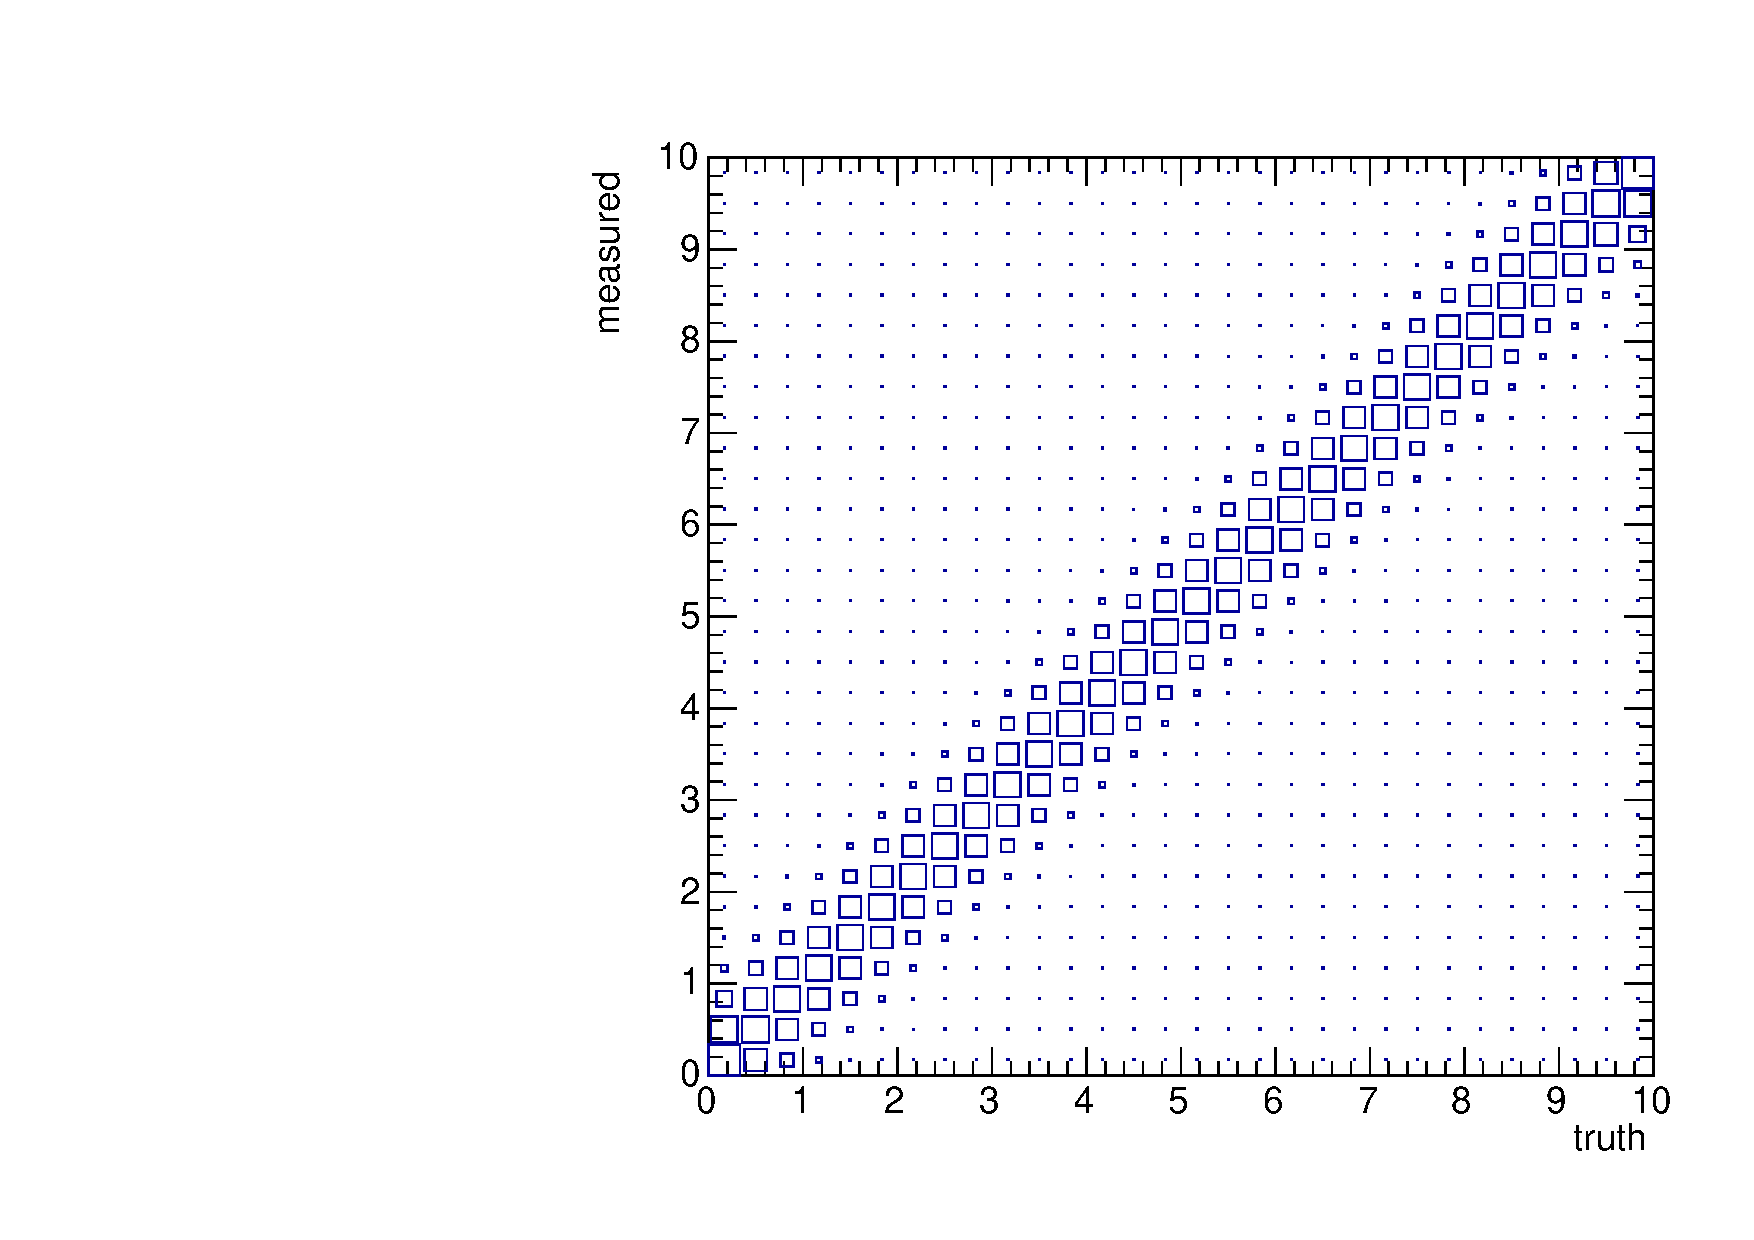
\includegraphics[width=0.49\textwidth]{figs/respt.pdf}
	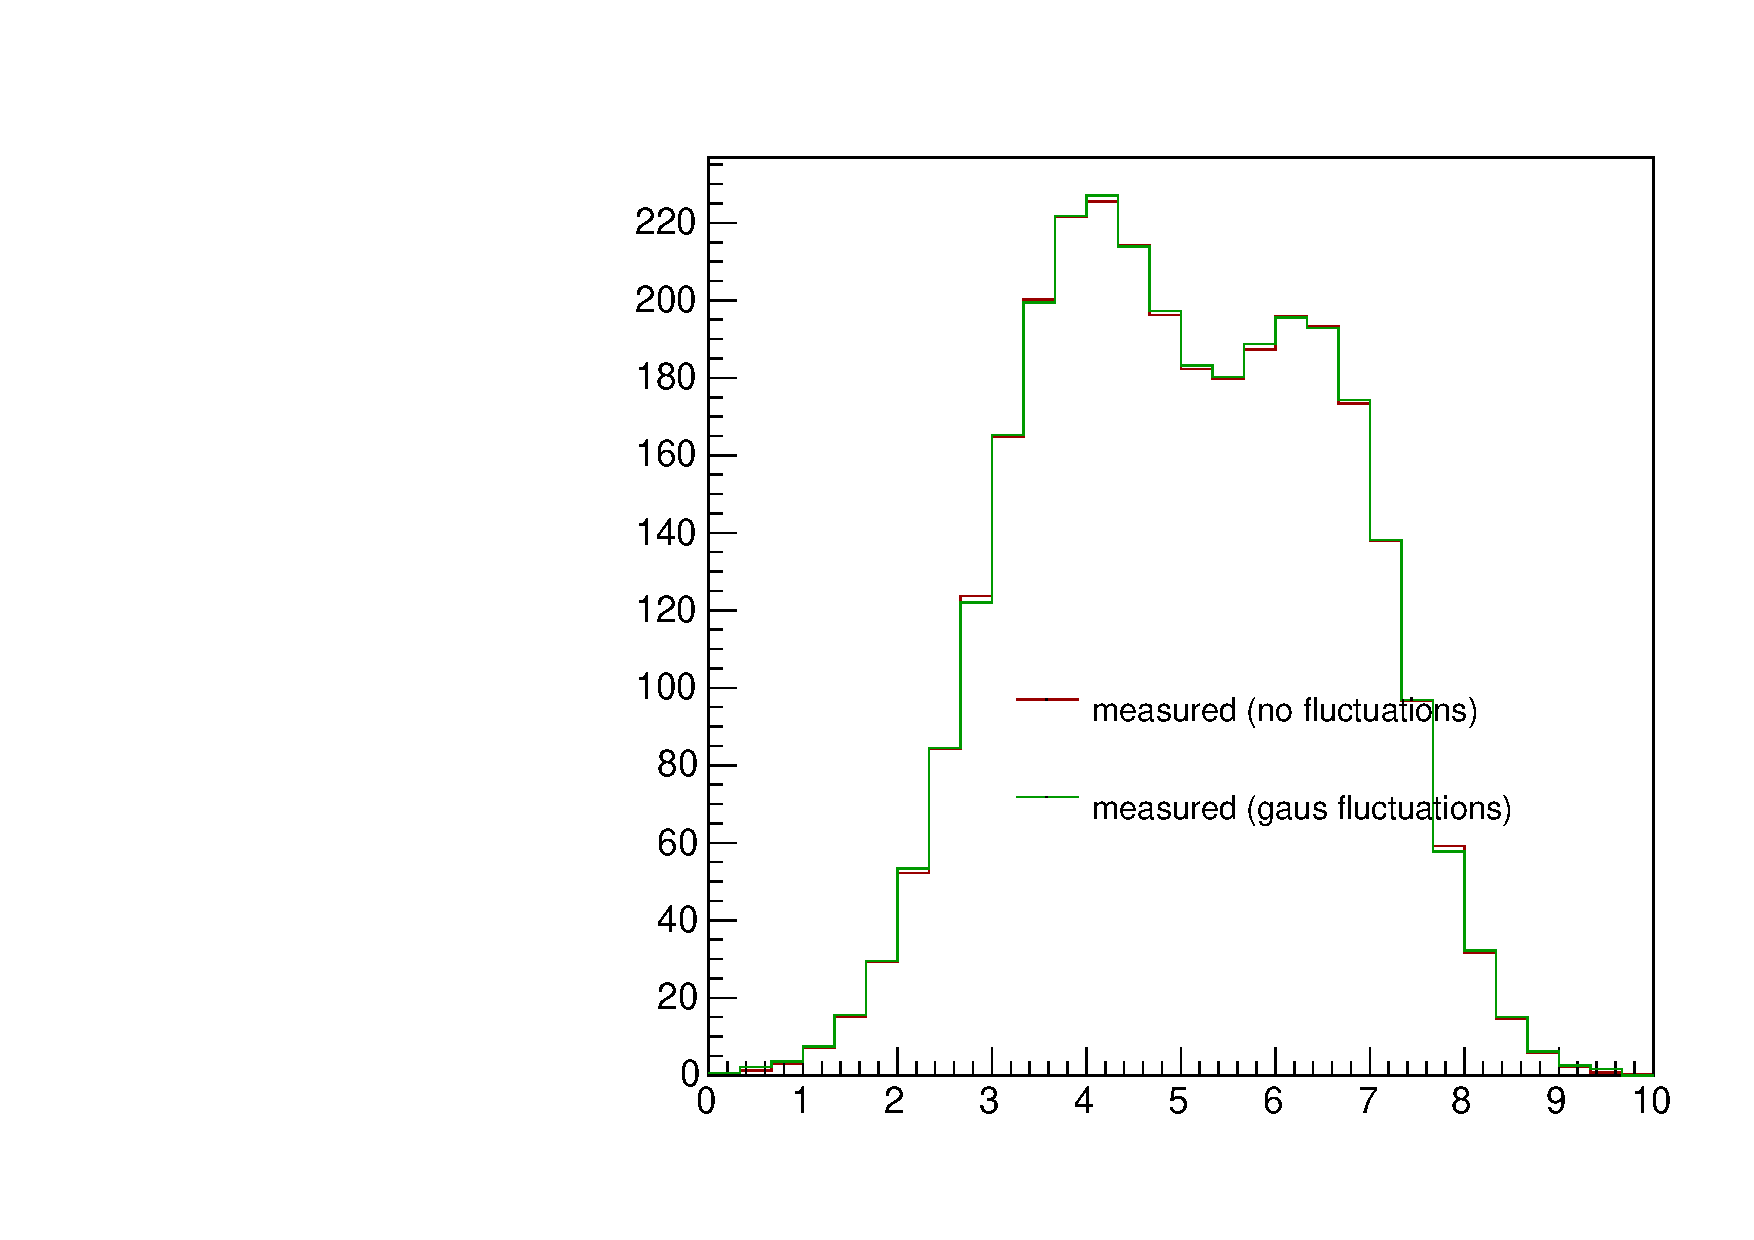
\includegraphics[width=0.49\textwidth]{figs/reco.pdf}
	\caption{
		\label{fig:exe1}
		Left: smearing matrix ($\respt$) 
		Right: reconstructed distributions with and without random fluctuations.
	}	
\end{figure}
\FloatBarrier

\section{Regularized Unfolding}
\difficulty{3}

The most used unfolding methods in \gls{HEP} are the iterative method based on Bayes' theorem \cite{dAgostini} and the \gls{SVD} method \cite{SVD}.
For the iterative method based on Bayes' theorem the regularization is given by the number of iteration, while for the \gls{SVD} method the regularization parameter is the number of singular values used in the inversion.

Using the histogram with fluctuations of the exercise above:
\begin{enumerate}
	\item provide a graphical representation of the unfolded distribution with different regularization parameters for both algorithms.
	\item discuss the effect and the limits of the regularization parameter in the two methods.
	\item discuss how you would choose the regularization parameter.
	\item discuss the pro and cons of the two methods.
\end{enumerate}

\section{Constructing a Response Matrix}
\difficulty{4}

The scope of this exercise is to simulate the unfolding of a $p_{T}^{Z}$ distribution with the $\mathrm{Z}$ 
boson decaying into a $\mu$-pair.
In general the response matrix is built from an event-based \gls{MC} simulation.
In this section the goal is to unfold a given distribution, constructing before the response matrix.

Event-based \gls{MC} simulations
are usually produced with different \emph{luminosity} that the one produced by the machine.
Often it happens that small region of the phase space that are interesting for searches and measurements have an enhanced size, 
leading to different per event weights.

Unfortunately, the \gls{MC} simulation is not perfect and needs to be corrected for small effects.
Typically these can be \emph{scale-factors} measured with the \emph{tag-and-probe} method. 
This type of weights aims to correct the difference in efficiency observed in the objects reconstruction
and are assumed to be uncorrelated between the different objects.

The {\scshape root} file (\verb@Exe2.root@) contains a list of \gls{MC} events inside a tree (\verb@Exe2.root/events@) with the following information:
\begin{itemize}
	\item The $p_\textup{T}$, $\eta$, $\phi$ of the two muons generated and reconstructed; 
	      When not said otherwise units are in GeV ($c=1$).
	\item An event weight given by the \gls{MC}-simulation. 
\end{itemize}
And a data distribution to unfold (\verb@Exe2.root/data@). 

The following fiducial cuts must be applied on both muons:
\begin{itemize}
	\item $p_\textup{T}^\mu >15 $ GeV 
	\item $|\eta^\mu| < 2.5 $
\end{itemize}

The \emph{scale-factors} ($\varepsilon_\textup{DATA} / \varepsilon_\textup{MC}$) for the muons efficiencies are given in the file 
\verb@scalefactors.txt@ for the corresponding $\eta$ and $p_\textup{T}$ ranges.

\vspace{1cm}

\begin{enumerate}
	\item Provide a {\scshape root} file with:
		\begin{itemize}
		\item the set of histogram used to build the response matrix.
			\begin{itemize}
			\item \verb@TH1D@ named \verb@matrix_measured@
			\item \verb@TH1D@ named \verb@matrix_truth@
			\item \verb@TH2D@ named \verb@matrix_matrix@ (with the truth bins on the $y$-axis and the measured ones on the $x$ axis)
			\end{itemize}
		\item  the unfolded distribution of the data, a \verb@TH1D@ with name \verb@data_unfold@
		\end{itemize}
	\item explain how you get the response matrixes, the unfolded distribution and the errors associated.
\end{enumerate}

%%%%%%%%%%%%%%%%%%%% BIBLIO %%%%%%%%%%%%%%%%%%%%%%
\FloatBarrier
\nocite{*}
%\bibliographystyle{acm}
\bibliographystyle{acmunsrt}
%\addcontentsline{toc}{section}{\refname}
\bibliography{UnfoldingExe}
%%%%%%%%%%%%%%%%%%
\cleardoublepage

\end{document}
